%% Kapitel Funktionen
%% GESO-Kompendium
%% philipp.freimann@bbw.ch
%%

\deu{\section{Funktionen}\index{Funktionen}}
\eng{\section{Functions}\index{Functions}}
\setcounter{aufgabenNummer}{1}
\renewcommand{\kAufgabenBuchstabe}{F}

\subsection{\deu{Grundlagen}\eng{Basics}}

\kTrainingAufgabe{
\eng{translate:}
\textbf{\deu{Graphen Zeichenen}\eng{Drawing graphs}}:
\deu{Zeichnen Sie den Graphen der Funktion im Bereich}
\eng{Sketch the graph of the function in the range}
$-4 \le{} x \le{} 4$.

a) $y=\frac12\cdot{}x$ \hspace{30mm}
b) $y=\frac1x$ \hspace{30mm}
c) $y=x^2$

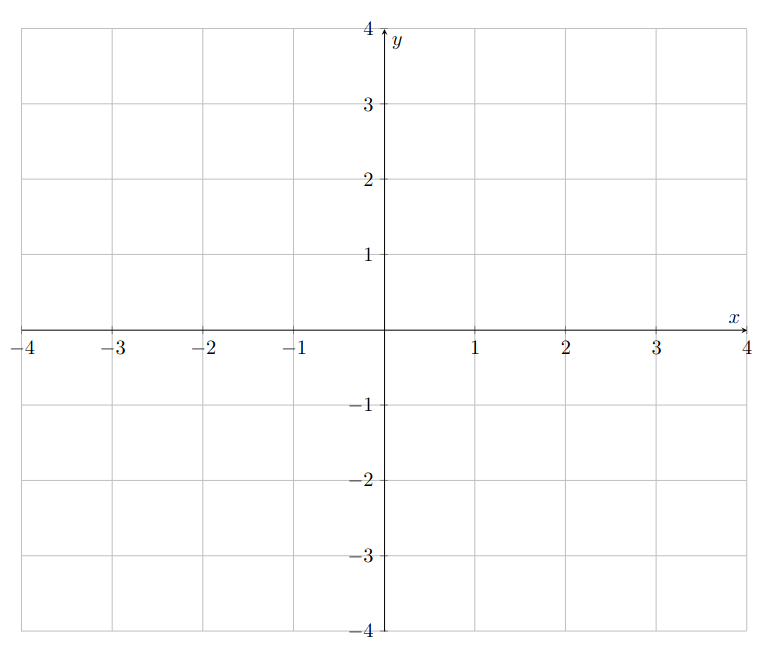
\includegraphics[width=150mm]{img/fct/Fct_ssA01.png}

}{%% Lösung
\raisebox{-80mm}{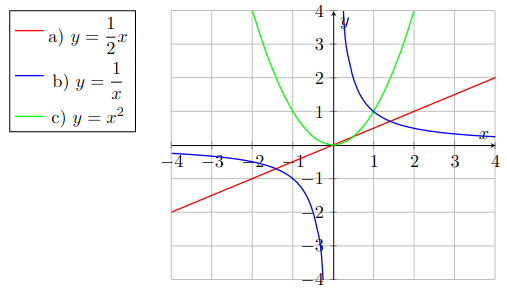
\includegraphics[width=150mm]{img/fct/Fct_ssL01.png}}
}{8}



\kTrainingAufgabe{
\eng{translate:}
\textbf{\deu{Funktionen auswerten}\eng{Evaluate the function}}:
\deu{Werten Sie den Funktionsterm $y=x^2-2x-5$ für folgende $x$-Werte aus:}
\eng{Evaluate the function term $y=x^2-2x-5$ for the following $x$-values:}

a) $\frac12$ \hspace{25mm}
b) $-1$ \hspace{25mm}
c) $-\frac12$ \hspace{25mm}
d) $-\frac34$ \hspace{25mm}

}{%% Lösung
a) $-\frac{23}4$ \hspace{25mm}
b) $-2$ \hspace{25mm}
c) $-\frac{15}{4}$ \hspace{25mm}
d) $-\frac{47}{16}$ \hspace{25mm}
}{8}

\subsection{\deu{Lineare Funktionen}\eng{Linear Functions}}

\kTrainingAufgabe{
\eng{translate:}
\textbf{\deu{Steigungsbegriff, Mittelpunkt einer Strecke}\eng{Slope concept, midpoint of a line segment}}:

\kKommentar{Mittelpunkt ist ein geometrisches Konzept.}
\kKommentar{Kommt im Rahmenlehrpln \textbf{nicht} vor?}

a) \deu{Bestimmen Sie die Steigungen der Strecken a bis i. Zeichnen Sie
Steigungsdreiecke ein.}
\eng{Determine the slopes of the line segments a to i. Draw slope triangles.}

b) \deu{Bestimmen Sie die Koordinaten des Mittelpunkts jeder Strecke.}
\eng{Determine the coordinates of the midpoint of each line segment.}

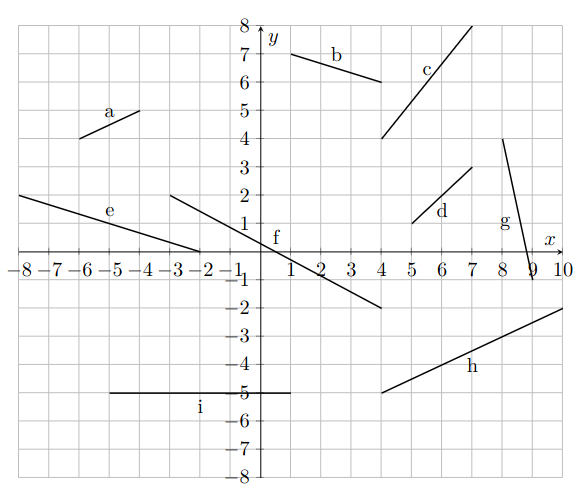
\includegraphics[width=130mm]{img/fct/Fct_ssA03.png}
}{%% Lösung

\renewcommand{\arraystretch}{2}
\begin{tabular}{|c|c|c|c|c|c|c|c|c|c|}\hline
   & a & b &c &d &e &f &g &h &i\\\hline
$a=m=$ & $\frac12$ & $\frac{-1}3$ & $\frac43$ & $1$ & $\frac{-1}3$
& $\frac{-4}7$ & $-5$ & $\frac12$ & $0$\\\hline
M.: & $(-5|\frac92)$ & $(\frac52|6.5)$ & $(5.5|6)$ & $(6|2)$ &
$(-5|1)$ & $(\frac12|0)$ & $(8.5|\frac32)$ & $(7|\frac{-7}2)$ & $(-2|-5)$\\\hline
 \end{tabular}
\renewcommand{\arraystretch}{2}
 
}{8}



%%% ab hier weiter übersetzen
\kTrainingAufgabe{
\eng{translate:}
\textbf{Graph zeichnen, Achsenschnittpunkte einzeichnen}:
Zeichnen Sie die Graphen folgen-
der Funktionen und heben Sie den Schnittpunkt mit der y-Achse und die Nullstelle hervor.
a) $y=2x+1$ \hspace{25mm}
b) $y=-x+3$ \hspace{25mm}
c) $y=-0.5x+4$ \hspace{25mm}

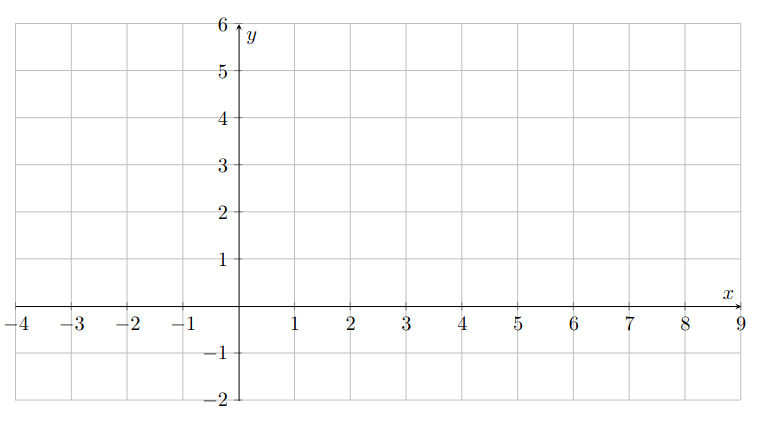
\includegraphics[width=150mm]{img/fct/Fct_ssA04.png}
}{%% Lösung

\raisebox{-50mm}{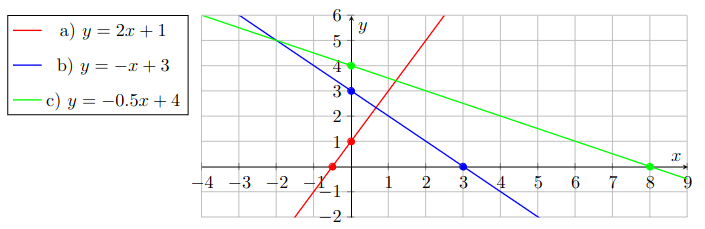
\includegraphics[width=150mm]{img/fct/Fct_ssL04.png}}

}{8}



\kTrainingAufgabe{
\eng{translate:}
\textbf{Funktionsterm auswerten:} Werten Sie die Funktion $f(x) = 2x+1$ für folgende Argumente
aus: $2$, $-2$, $0.5$, $-0.5$.
}{%% Lösung
$f(2)= 5$ \hspace{10mm}
$f(-2)=-3$ \hspace{10mm}
$f(0.5) = 2$ \hspace{10mm}
$f(-0.5)=0$
}{8}





\kTrainingAufgabe{
\eng{translate:}
\textbf{Bedeutung der Parameter; explizite Form:} Bestimmen Sie Steigung und $y$-
Achsenabschnitt in der durch die Funktionsgleichung $3x-2y=60$ gegebenen Geraden.

}{%% Lösung
$$y = 1.5x - 30$$
Steigung = 1.5 und $y$-Achsenabschnitt = -30.
}{8}





\kNiveauAufgabe{
\eng{translate:}\textbf{Achsenschnittpunkte berechnen:}
Berechnen Sie die Achsenschnittpunkte der Geraden $g$
mit der Funktionsgleichung $y=-0.25x+4$.
}{%% Lösung
Mit $x$-Achse: $(0|4)$

Mit $y$-Achse: $(16|0)$
}{8}





\kTrainingAufgabe{
\eng{translate:}\textbf{Horizontale Gerade:}
Notieren Sie die Funktionsgleichung der horizontalen Geraden durch den Punkt $P=(5|8)$.
}{%% Lösung
$f(x) = y = 8$
}{8}





\kNiveauAufgabe{
\eng{translate:}\textbf{Zweipunkteaufgabe:}
Wie lautet die Funktionsgleichung der Geraden, die durch folgende
zwei Punkte läuft (Resultate exakt angeben)?

a) $A(5|8)$ und $B(7|12)$


b) $A(-3|4)$ und $B(2|1)$


c) $A(-1|1)$ und $B(10|5)$

}{%% Lösung
a) $A=(5|8)$ und $B=(7|12)$ $\Longrightarrow$  $y=2x-2$


b) $A=(-3|4)$ und $B=(2|1)$ $\Longrightarrow$ $y=\frac{-3}5x+\frac{11}5$


c) $A=(-1|1)$ und $B=(10|5)$ $\Longrightarrow$  $y=\frac4{11}x+\frac{15}{11}$
}{8}




\kTrainingAufgabe{
\eng{translate:}\textbf{Funktionsgleichung aus Grafik bestimmen}
Wie lauten die Funktionsgleichungen der Geraden $a$ bis $f$?

\kKommentar{Niveau Aufnahmeprüfung!}

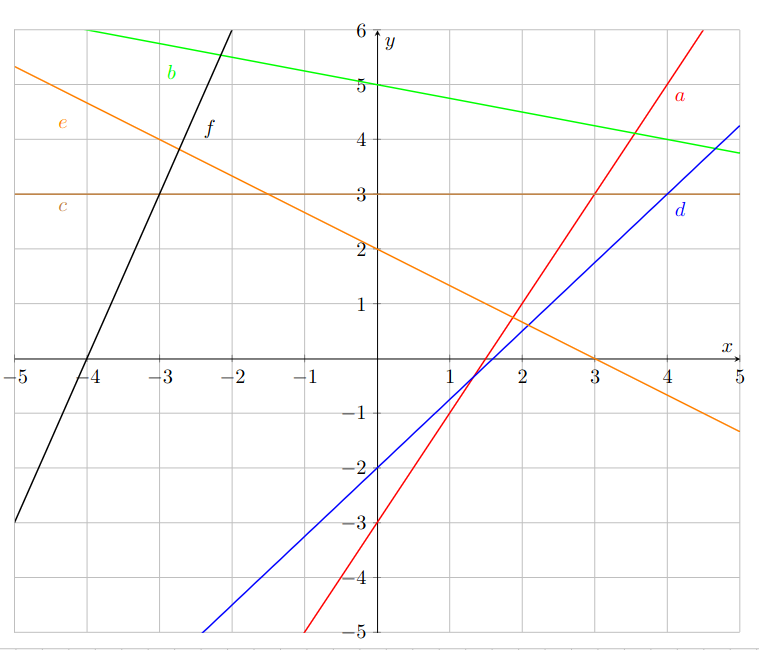
\includegraphics[width=140mm]{img/fct/Fct_ssA10.png}

}{%% Lösung
\raisebox{-80mm}{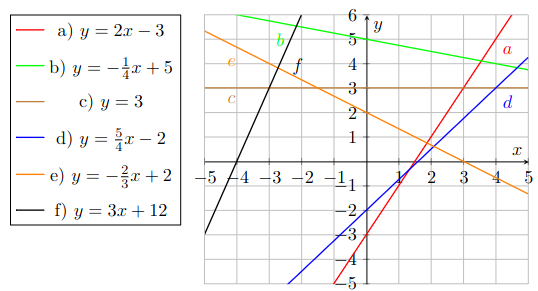
\includegraphics[width=160mm]{img/fct/Fct_ssL10.png}}
}{8}





\kNiveauAufgabe{
\eng{translate:}\textbf{Achsenschnittpunkte berechnen}
Berechnen Sie die Schnittpunkte des Graphen mit den beiden
Koordinatenachsen.

a) $y=10-3x$ \hspace{30mm}
b) $y=5-\frac12x$ \hspace{30mm}
c) $y=\frac{10x-2}5$ 
}{%% Lösung

\renewcommand{\arraystretch}{2}
\begin{tabular}{c|c|c|c}
& a) $y=10-3x$ & b) $y=5-\frac12x$ & c) $y=\frac{10x-2}5$  \\\hline
$N(x_n|0)$ & $\left(\frac{10}3\middle|0\right)$ & $(10|0)$ &
$(\frac15|0)$ \\\hline
$B(0|b)$ & $(0|10)$ & $(0|5)$ & $\left(0\middle|\frac{-5}2\right)$
 \end{tabular}
 
\renewcommand{\arraystretch}{2}

}{8}






\kTrainingAufgabe{
\eng{translate:}\textbf{Umwandeln in die explizite Form}
Wandeln Sie die Funktionsgleichung in die explizite Form $y=ax+b$
(bzw. $y=mx+q$) um.

a) $y=2-\frac{x}2$

b) $y=\frac{2x-10}3$

c) $y=\frac{1-x}{12}$

d) $y = -(2+1.25x)$

e) $4y-3x = 1.5$
}{%% Lösung

a) $y=\frac{-1}2\cdot{}x + 2$

b) $y=\frac23\cdot{}x - \frac{10}3$

c) $y=\frac{-1}{12}\cdot{}x + \frac1{12}$

d) $y=\frac{-5}4\cdot{}x - 2$

e) $y=\frac34\cdot{}x + \frac38$
}{8}





\kNiveauAufgabe{
\eng{translate:}\textbf{Liegt $P (-4.5|7)$ auf, oberhalb oder unterhalb der Geraden $g$?}

a) $g: y=-2x-2$

b) $g: y= -0.5x + 4.7$

c) $g: y = 2.5x + 18.25$
}{%% Lösung

a) Punkt liegt \textbf{auf} der Geraden.  

b) Punkt liegt \textbf{oberhalb} der Geraden.  

c) Punkt liegt \textbf{auf} der Geraden.  

}{8}




\kNiveauAufgabe{
\eng{translate:}\textbf{Geradengleichung aus Steigung und einem Punkt
$P \in g$ (Punkt-Steigungs-Aufgabe)}

Eine Gerade $g$ hat die Steigung $-0.4$ und geht durch $P (-2| -7)$. Wie lautet
die Funktionsgleichung von $g$?
}{%% Lösung
$g : y = -0.4x - 7.8$
}{8}




\kNiveauAufgabe{
\eng{translate:}\textbf{Liegen drei gegebene Punkte auf einer gemeinsamen Geraden oder nicht?}
Liegen $A(-2.5| -20.8)$, $B(21.5|50.0)$ und $C(100.0|281.575)$ auf
einer gemeinsamen Geraden $g$ oder nicht? Begründung?
}{%% Lösung
Ja, die Steigung von $AB$ ist gleich der Steigung von $BC$, nämlich $2.95$.
}{8}




\kNiveauAufgabe{
\eng{translate:}\textbf{Fehlende Punktkoordinate bestimmen: }
Der Punkt $C(-12.5|y_C)$ liegt auf der Geraden
$g$ durch $A(-2.5| - 20.8)$ und $B(21.5|50.0)$. Wie lautet die Koordinate $y_C$?
}{%% Lösung

$y_C = -50.3$
}{8}




\kNiveauAufgabe{
\eng{translate:}\textbf{Geradengleichung einer zur gegebenen Geraden parallelen Geraden durch einen
Punkt bestimmen:}
Gegeben ist $g : y = 4.8x - 2$. Die Gerade $h$ ist parallel zu $g$ und läuft
durch den Punkt $P(-8|2)$. Wie lautet die Geradengleichung von $h$?
}{%% Lösung
$h : y = 4.8x + 40.4$
}{8}




\kNiveauAufgabe{
\eng{translate:}\textbf{Schnittpunkt S zweier Geraden berechnen:}

Berechnen Sie den Schnittpunkt von $g: \frac{-2}3x+5$ und $h: \frac{-3}4x+10$
}{%% Lösung
Schnittpunkt = $(180|125)$
}{8}



\textbf{Kombinationen obiger Grundaufgaben}

\kNiveauAufgabe{
\eng{translate:}Die Gerade g hat die Steigung $-0.5$ und die Nullstelle bei $x = 5$. Wie lautet die Funktions-
gleichung von $g$?

}{%% Lösung
$g : y = -0.5x + 2.5$
}{8}




\kNiveauAufgabe{
\eng{translate:}Die Gerade $g$ hat die Steigung $-3$. Ferner liegt $A(-2|4)$ auf $g$. Der Punkt $B(x_B | - 23)$ liegt
ebenfalls auf $g$. Wie lautet die Koordinate $x_B$?

}{%% Lösung
$x_B = 7$
}{8}




\kNiveauAufgabe{
\eng{translate:}Die Gerade $g$ geht durch $A(1|5)$ und $B(8| - 2)$. Die Gerade $h$ schneidet die $x$-Achse im
selben Punkt $N$ wie die Gerade $g$. Die Gerade $h$ hat ferner die Steigung $4$. Wie lautet die
Funktionsgleichung von $h$?

}{%% Lösung
$h : y = 4x - 24$
}{8}


\textbf{Angewandte lineare Funktionen}

\kNiveauAufgabe{
\eng{translate:}Eine Taxifahrt von 10 km kostet CHF 21, eine solche von 15 km aber CHF 27. Wie lautet
die lineaer Funktionsgleichung $y = f (x)$ mit $x$ = Anzahl km Fahrstrecke und $y$ = Anzahl CHF
Gesamttaxe? Variante: Gesucht die Funktionsgleichung $K = f (s)$, $K$ = Kosten in CHF, $s$ =
Strecke in km. Es werden beide Varianten akzeptiert.

}{%% Lösung

$y = 1.2x + 9 $

oder (Variante)

$K(s) = 1.2 \text{CHF/km} · s + 9 \text{CHF}$

}{8}





\kNiveauAufgabe{
\newcommand{\tempGrad}[1]{${}^{\circ{}}$#1}
\eng{translate:}Die englische Temperaturskala (Fahrenheit-Grade, \tempGrad{F}) ist wie folgt festgelegt:
0\tempGrad{C} (Celsius) entsprechen 32 \tempGrad{F} (Fahrenheit). 100 \tempGrad{C}
entsprechen 212 \tempGrad{F}.

a) Wie lautet die lineare Funktionsgleichung zur Umrechnung
von \tempGrad{C} (= $x$) in \tempGrad{F} (= $y$)?

b) Wie lautet die lineare umgekehrte Funktion zur Umrechnung von \tempGrad{F}(= $x$) in \tempGrad{C} (= $y$)?

}{%% Lösung
a) $y = 1.8x + 32$

b) $y= \frac95 x - \frac{160}9$
}{8}





\kNiveauAufgabe{
\eng{translate:}
Eine lineare Notenskala ist wie folgt festgelegt:
Für 24 Punkte gibt es Note 6, für 0 Punkte Note 1.

a) Wie lautet die lineare Notenfunktion $y = f (x)$? $x$ = Anzahl Punkte, $y$ = Notenzahl.

b) Welche Note (auf 1 Dezimale gerundet) wird mit 18 Punkten erreicht?

c) Wie viele Punkte ergeben die Note 4?
}{%% Lösung

a) $y=\frac5{24}x+1$

b) $4.8$

c) 14.4 Punkte
}{8}





\kNiveauAufgabe{
\eng{translate:}\textbf{}
Lineare Abschreibung einer Maschine: Eine Maschine mit Neuwert CHF 5’000.- wird linear
abgeschrieben: Jedes Jahr soll sich ihr Wert um CHF 250.- verringern.

a) Wie lautet die lineare Abschreibungsfunktion $y = f (x)$ mit $x$ = Anzahl Jahre und $y$ =
Anzahl CHF Zeitwert nach $x$ Jahren?

b) Nach wie vielen Jahren ist die Maschine vollständig abgeschrieben?
}{%% Lösung

a) $y = -250x + 5000$

b) Nach 20 Jahren.
}{8}





\kNiveauAufgabe{
\eng{translate:}\textbf{}
Für HD-TV via Internet wird neben einer Grundgebühr auch die Anzahl Stunden, während
derer man fernsieht, verrechnet. Anbieter A verlangt pro Monat eine Grundgebühr von CHF
5.- und pro Stunde fernsehen eine Gebühr von 20 Rappen. Anbieter B verlangt folgendes:
Bei 20 h fernsehen CHF 10.- und bei 100 h fernsehen CHF 20.- (beides inkl. Grundgebühr).
Wie lauten die beiden Kostenfunktionen? $x$ = Anzahl Stunden Fernsehzeit, $y$ = Anzahl CHF
Kosten. Bei welcher Stundenzahl sind beide Anbieter gleich teuer?
}{%% Lösung
Gleicher Preis bei 33 Stunden und 20 Minuten.
}{8}



\subsubsection{Grafisches Lösen von Gleichungssystemen}


\kNiveauAufgabe{
\eng{translate:}
Lösen Sie das Gleichungssystem grafisch und interpretieren Sie die
Lösung:

a) \gleichungZZ{3x-4y}{8}{y}{\frac14 x + 6}

\begin{center}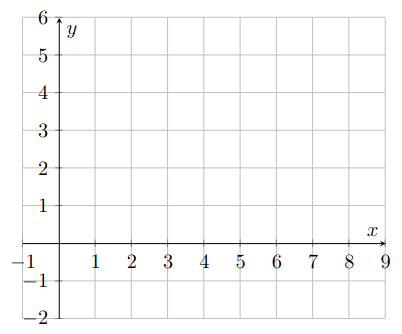
\includegraphics[width = 100mm]{img/fct/Fct_ssA27a.png}\end{center}


b) \gleichungZZ{10y}{7.5x}{18.75x+25y}{1500}

\begin{center}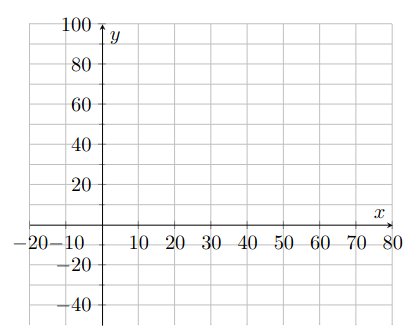
\includegraphics[width = 100mm]{img/fct/Fct_ssA27b.png}\end{center}

c) \gleichungZZ{13x+y-9.5}{4y-\frac{28}7}{-\frac45y+x}{-5+0.2x}

\begin{center}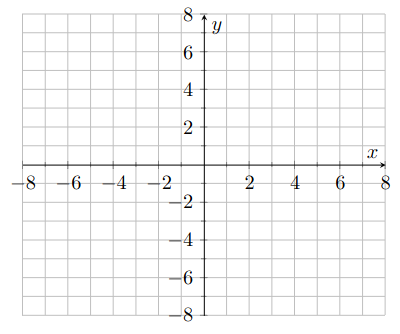
\includegraphics[width = 100mm]{img/fct/Fct_ssA27c.png}\end{center}

d) \gleichungZZ{40}{-2y-x}{3.5x-5y+82}{4\left(x-y+\frac{51}2\right)}

\begin{center}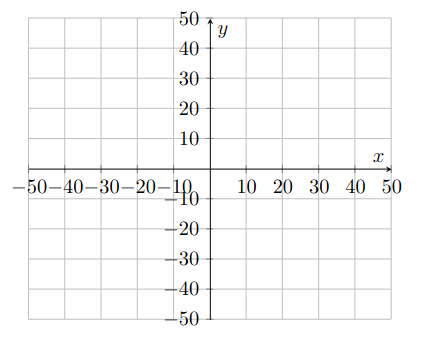
\includegraphics[width = 100mm]{img/fct/Fct_ssA27d.png}\end{center}

}{%% Lösung

a) \gleichungZZ{3x-4y}{8}{y}{\frac14 x + 6} $$S=(8|4)$$

\begin{center}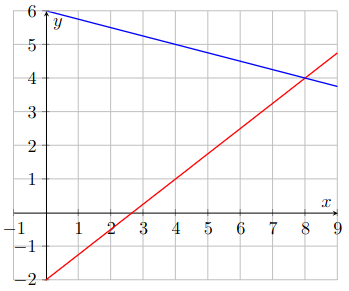
\includegraphics[width = 100mm]{img/fct/Fct_ssL27a.png}\end{center}


b) \gleichungZZ{10y}{7.5x}{18.75x+25y}{1500} $$S=(40|30)$$

\begin{center}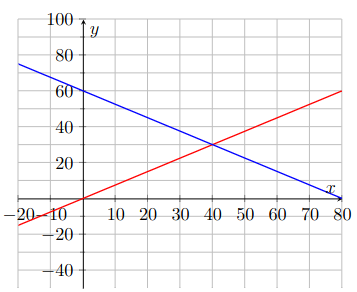
\includegraphics[width = 100mm]{img/fct/Fct_ssL27b.png}\end{center}

c) \gleichungZZ{13x+y-9.5}{4y-\frac{28}7}{-\frac45y+x}{-5+0.2x}

$$\mathbb{L}_S = \left\{\right\}$$

\begin{center}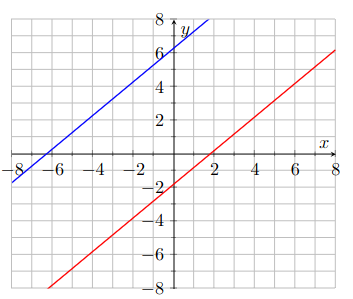
\includegraphics[width = 100mm]{img/fct/Fct_ssL27c.png}\end{center}

d) \gleichungZZ{40}{-2y-x}{3.5x-5y+82}{4\left(x-y+\frac{51}2\right)}

Die Geraden sind zusammenfallend. 

\begin{center}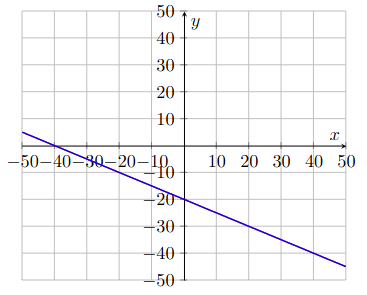
\includegraphics[width = 100mm]{img/fct/Fct_ssL27d.png}\end{center}

}{2}
\newpage






\subsection{\deu{Potenzfunktionen}\eng{Power Functions}}
\kKommentar{Graphen von Potenzfunktionen sind Hyperbeln oder
  Parabeln...}
  
\kKommentar{...Dies in den Titeln korrekt vermerken (nicht
  Hyperbelfunktion etc.)}

\subsubsection{$n>1$: \deu{Parabeln}\eng{Parabolas}}

\kNiveauAufgabe{
\deu{Zeichnen Sie den Graphen folgender Potenzfunktionen:}
\eng{Draw the graph of the following power functions:}
a) $x \mapsto 0.5x^3$  \hspace{30mm}  b) $x\mapsto -x^4$

\begin{tabular}{cc}
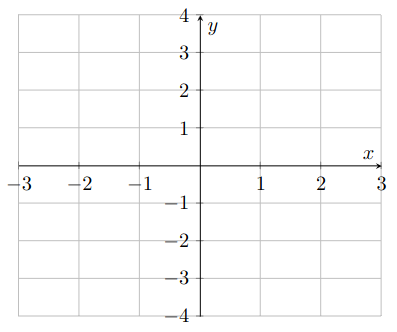
\includegraphics[width=85mm]{img/fct/Fct_ssA28a.png}
&
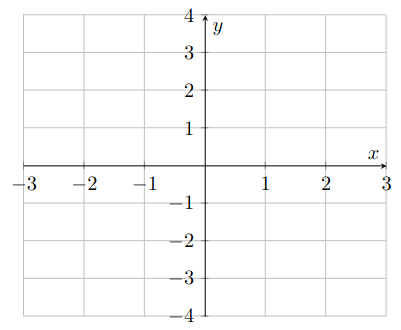
\includegraphics[width=85mm]{img/fct/Fct_ssA28b.png}
\\
 \end{tabular}
 

}{%% Lösung

\begin{tabular}{cc}
a)

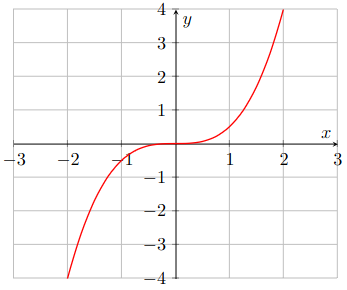
\includegraphics[width=70mm]{img/fct/Fct_ssL28a.png}
&b)

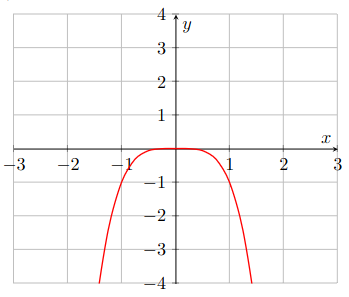
\includegraphics[width=70mm]{img/fct/Fct_ssL28b.png}
\\
 \end{tabular}

}{4}


\kNiveauAufgabe{
\deu{Bestimmen Sie den Faktor $a$ in $x\mapsto a\cdot{}x^4$ wenn der Graph durch den Punkt $A(3|3)$ verläuft.}
\eng{Determine the factor $a$ in $x\mapsto a \cdot x^4$ when the graph
passes through the point $A(3|3)$.}
}{%% Lösung
$3=3\cdot{}a^4 \Longrightarrow a=\frac1{27}$
}{6}%% end KNiveauAufgabe




\subsubsection{$n < 0$ \deu{Hyperbeln}\eng{Hyperbolas}}\index{\deu{Hyperbeln}\eng{Hyperbolas}}



\kNiveauAufgabe{
\deu{Bestimmen Sie den Faktor $a$ der Potenzfunktion $y=a\cdot{}x^{-3}$,
wenn der Graph dieser Hyperbel durch den Punkt
$A\left( 3 \middle| \frac1{54} \right)$ verläuft.}
\eng{Determine the factor $a$ of the power function $y = a \cdot x^{-3}$ when the graph of this hyperbola passes through the point $A\left(3 \middle| \frac{1}{54}\right)$.}
}{%% Lösungs
$\frac1{54}=a\cdot{}3^{-3} \Longrightarrow   a=27\cdot{}\frac1{54} = \frac12$
}{8}









\kNiveauAufgabe{
\deu{Welche Funktion gehört zu welchem Graphen? Ordnen Sie die Zahl dem Buchstaben zu.}
\eng{Which function belongs to which graph? Match the number to the letter.}

a) $y = -x^3$  \hspace{15mm}  b) $y=x^{-2}$  \hspace{15mm} c)
$y=3\cdot{}x^{-1}$ \hspace{15mm}  d) $y=-0.5x^4$

\begin{center}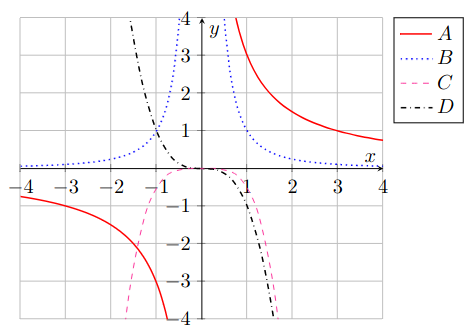
\includegraphics[width=150mm]{img/fct/Fct_ssA31.png}\end{center}

}{%% Lösung
a) $y = -x^3$  \hspace{15mm}  b) $y=x^{-2}$  \hspace{15mm} c)
$y=3\cdot{}x^{-1}$ \hspace{15mm}  d) $y=-0.5x^4$

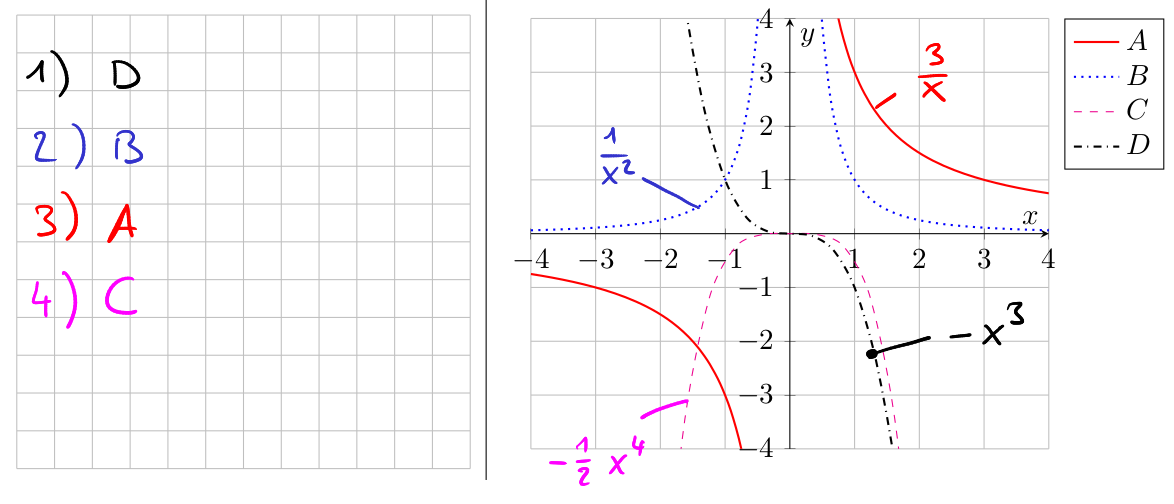
\includegraphics[width=150mm]{img/fct/Fct_ssL31.png}

}{4}

\newpage







\subsection{\eng{translate: }Exponentialfunktionen}

\newcommand{\e}{\text{e}}
\subsubsection{\eng{translate: }Exponentielle Prozesse, Exponentialfunktion}

\textbf{\eng{translate: }Wachstums und Zerfallsprozesse}

\kNiveauAufgabe{
\deu{Zinseszins; Entwicklung eines Startkapitals bei konstantem Jahreszinssatz: Ein
Kapital von CHF 100.- wird über viele Jahre zu einem konstanten
\eng{Zinssatz von 2\% verzinst.}Compound interest; development of an initial capital with a constant annual interest rate: A capital of CHF 100.- is compounded over many years at a constant interest rate of 2\%.}

\begin{enumerate}[label=\alph*)]
\item
\deu{Bestimmen Sie den Zinsfaktor.}\eng{Bestimmen Sie den Zinsfaktor.}
\item
\deu{Wie lautet die Funktion $K = f (t)$, $K$ = Kapital zur Zeit $t$,
$t$ = Zeit in Jahren?}
\eng{What is the function $K = f(t)$, where $K$ is the capital at time $t$, and $t$ is the time in years?}

\item
\deu{Stellen Sie die Kapitalentwicklung grafisch dar}%
\eng{Graphically represent the capital development}:
$0 \le t \le 320$.
\end{enumerate}

\begin{center}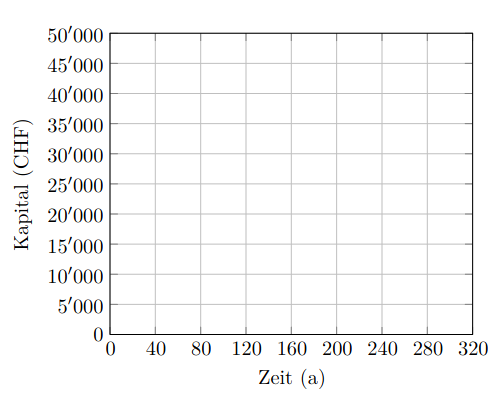
\includegraphics[width=150mm]{img/fct/Fct_ssA32.png}\end{center}


}{%% Lösung
\begin{enumerate}[label=\alph*)]
\item
Der Zinsfaktor ist $1.02$.
\item
$K = f (t) = 100\cdot 1.02 ^ t$, $t$ = Zeit in Jahren?
\item
\deu{S. folgende Grafik}
\eng{consult the following graphic}
\end{enumerate}
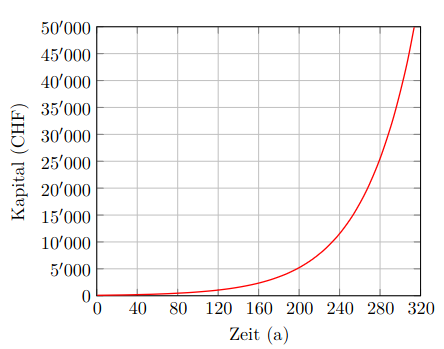
\includegraphics[width=150mm]{img/fct/Fct_ssL32.png}

}{8}





\kNiveauAufgabe{
\eng{translate:} Degressive Abschreibung:
Eine Maschine mit einem Neuwert von CHF 20\,000.- wird de-
gressiv abgeschrieben. Sie verliert jährlich 10\% an Wert.
\begin{enumerate}[label=\alph*)]
\item
 Bestimmen Sie den Abnahmefaktor.
\item
 Erstellen Sie eine Wertetabelle: $t$ = Zeit in Jahren, $W=f(t)$ = Wert Maschine zur Zeit $t$.
\item
 Stellen Sie die Werte-Entwicklung grafisch dar: $0 \le t \le 10$.
\item
 Wie lautet eine möglicher Funktionsterm zu $W=f(t)$?
\end{enumerate}

\begin{center}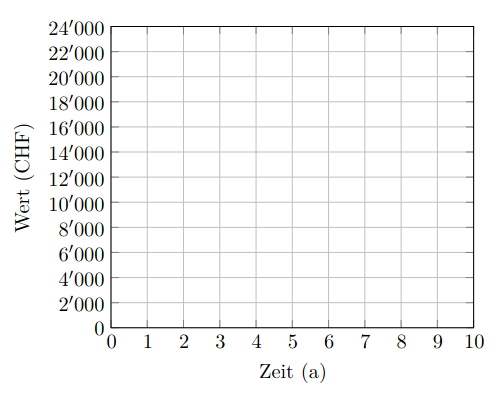
\includegraphics[width=150mm]{img/fct/Fct_ssA33.png}\end{center}
}{%% Lösungen
\begin{enumerate}[label=\alph*)]
\item
Der Abnahmefaktor (hier Abschreibungsfaktor) ist $100\%-10\% =
(100-10)\% = 90\% = 90\cdot{}\frac1{100} = 0.9$
\item
\begin{tabular}{|c|c|c|c|c|c|}\hline
Jahr   & 0 & 1 & 2 & 3 & 4 \\\hline
Wert   & 20\,000 & 18\,000 & 16\,200 & 14\,580 & 13\,122 \\\hline
 \end{tabular}
 
\item
\deu{S. folgende Graphik}
\eng{consult the following graphic}
\end{enumerate}
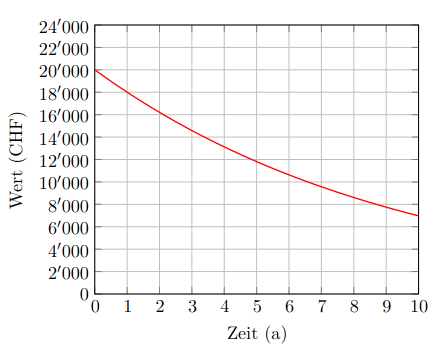
\includegraphics[width=150mm]{img/fct/Fct_ssL33.png}

}{}


\kTrainingAufgabe{
\eng{translate:} Prozentuale Wachstumsrate $\leftrightarrow$
Wachstumsfaktor: Suchen Sie zu folgenden
prozentualen Wachstumsraten den zugehörigen Wachstumsfaktor:

a) Rate = $4\%$
\hspace{15mm}
b) Rate = $2.2\%$
\hspace{15mm}
c) Rate = $0.5\%$
}{%% Lösungen

a) $1.04$ 
\hspace{15mm}
b) $1.022$
\hspace{15mm}
c) $1.005$
}{4}


\kTrainingAufgabe{
\eng{translate:} Prozentuale Abnahmerate $\leftrightarrow$ Abnahmefaktor: Suchen Sie zu folgenden prozentualen
Abnahmeraten den zugehörigen Abnahmefaktor:

a) Rate = $4\%$
\hspace{15mm}
b) Rate = $20\%$
\hspace{15mm}
c) Rate = $5.5\%$
}{%% Lösungen

a) $0.96$ 
\hspace{15mm}
b) $0.8$
\hspace{15mm}
c) $0.945$
}{4}



\newpage
\kNiveauAufgabe{
\eng{tranlate:}
\textbf{Graphen von Exponentialfunktionen:}

Zeichnen Sie die Graphen von $f(x) = 2^x$ und $g(x) = 2^{-x}$ im
Bereich $-3 \le x \le 3$.

a) Vergleichen Sie die beiden Graphen. Wo schneiden sich die Graphen?

b) Bestimmen Sie Definitionsbereich und Wertebereich der beiden Funktionen.

c) Haben die Funktionen Nullstellen? Haben Sie Asymptoten?

\bbwGraph{-4}{4}{-1}{9}{}

}{%% Lösung
\begin{center}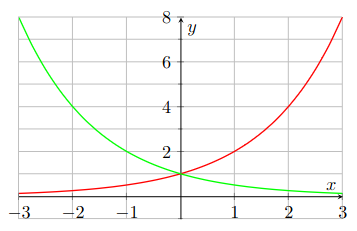
\includegraphics[width=150mm]{img/fct/Fct_ssL36.png}\end{center}

a) Die Graphen sind spiegelsymmetrisch (gespiegelt an der
$y$-Achse. Sie schneiden sich im Punkt $(0|1)$.

b) Definitonsbereich $\mathbb{D} = \mathbb{R}$ und Wertebereich
$\mathbb{W} = \mathbb{R}^{+}\backslash \{0\}$.

c) Die Funktionen haben keine Nullstellen, da der Wertebereich
$\mathbb{R}^+\backslash{}\{0\}$ ist. Der Funktions\textbf{wert} Null
kommt also nicht vor.

Für beide Funktionen ist die $x$-Achse die Asymptote.
}{4}

\kNiveauAufgabe{
Nennen Sie eine mögliche Exponentialfunktion $f(x) = a^x$ (also mit $f(0)=1$), bei der sich der Funktionswert

a) verdoppelt, wenn man das Argument um 3 erhöht (siehe Abbildung),

\begin{center}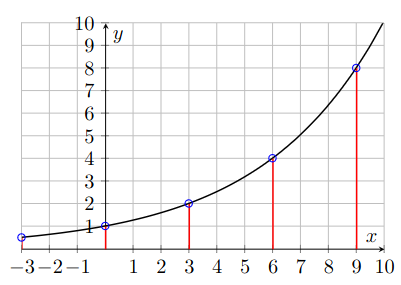
\includegraphics[width=65mm]{img/fct/Fct_ssA37.png}\end{center}

b) verdoppelt, wenn man $x$ um 12 erhöht bzw.

c) halbiert, wenn man $x$ um 12 erhöht.


}{%% Lösung
a) $f(x) = 2^\frac{x}3 =  \left(2^\frac13\right)^x
=\left(\sqrt[3]{2}\right)^x  $

b) $f(x) = 2^\frac{x}{12} =  \left(2^\frac1{12}\right)^x
=\left(\sqrt[12]{2}\right)^x  $

b) $f(x) = \left(\frac12\right)^\frac{x}{12} =  \left(\left(\frac12\right)^\frac1{12}\right)^x
=\left(\sqrt[12]{\frac12}\right)^x  $

}{8}


\kNiveauAufgabe{
\eng{translate:}

a) Die Wachstumsrate der Bevölkerung in der Schweiz betrug im Jahr 2012 ca. 1.1\%. 2012
zählte die Schweiz 8\,039\,100 Einwohner. Wie viele Personen werden bei gleich bleibender
Wachstumsrate im Jahr 2030 in der Schweiz leben (auf 100 Personen
genau)?

b) Seit 1999 wächst die Wohnbevölkerung der Stadt Zürich wieder. Im Jahr 1999 zählte die
Stadt Zürich 360\,704 Einwohner, im Jahr 2012 waren es 394\,012 Personen. Berechnen Sie
die durchschnittliche jährliche Wachstumsrate in \% (Genauigkeit: 2 Dezimalen). (Zum
Vergleich: Im Jahr 2012 betrug die Wachsumsrate 1\%.)
}{%% Lösungen

a) $8\,039\,100 \cdot{} 1.011^t$ mit $t=2030-2012=18$ ist $9\,788\,800$.

b) $\Delta\tau = 2012-1999 = 13$, somit gilt für die Wachstumsrate
$$q^{13} = \frac{394\,012}{360\,704} \Longrightarrow
q=\sqrt[13]{...}\approx 1.0068$$
Somit beträgt die jährliche Wachstumsrate ca. 0.68\%.
}{8}


\kNiveauAufgabe{\eng{translate:}
Berechnen Sie die durchschnittliche jährliche Wachstumsrate in \% für die Bevölkerung einer
Stadt, die innert 10 Jahren von 70’000 Personen auf 82’000 Personen angewachsen ist. (Ge-
nauigkeit: 1 Dezimale.)
}{%% Lösung
$\Delta\tau = 10$ somit gilt für den Wachstumsfaktor
$q^{10} = \frac{82\,000}{70\,000}$. Der Faktor ist daher $q=\sqrt[10]{\frac{82}{70}} \approx 1.0159$. Die
prozentuale Zunahme (Rate) gerundet in Prozent ist also: 1.6\%.

}{8}



\kNiveauAufgabe{\eng{translate:}

\kKommentar{Aufgabe geändert, da Begriff Eindringtiefe schon vergeben}

\kKommentar{Eindringtiefe $d= 1/\ln(a)$ mit $a$=Abnahmefaktor pro cm.}

Licht, das durch eine Glasplatte der Dicke $d$ geht, verliert an Intensität $I$. 
Pro eingedrungenen cm verliert das Licht bei einer bestimmten
Glassorte 60\% seiner Intensität. Die
Anfangsintensität beträgt 100 Watt/m${}^2$.

a) Bestimmen Sie eine mögliche Funktionsgleichung $I = f(d)$, für $I$ =
Intensität in W/m${}^2$ und $d$ = cm der Eindringung.

b) Bestimmen Sie die Intensität nach 5 cm im Glas. (Genauigkeit 3 Dezimalen.)

c) Nach wie vielen cm im Glas beträgt die Lichtintensität noch 1/100 der Anfangsin-
tensität? (Genauigkeit: auf mm genau.)

}{%% Lösungen

a) $I = f(d) =
100\cdot{}0.4^d \left[\frac{\text{Watt}}{\text{m}^2}\right]$

b)  $f(5) = 0.4^5 = 1.024 \left[\frac{\text{Watt}}{\text{m}^2}\right]$

c) $\log_{0.4}\left(\frac1{100}\right) \approx 5.026$ cm. Gerundet: 50 mm
}{8}


\kNiveauAufgabe{\eng{translate:}
Bei der Radio-Iodtherapie kommt radioaktives ${}^{131}$Iod zum Einsatz. Von anfänglich 20.000 mg
Substanz sind nach 7 Tagen noch 10.289 mg vorhanden.

a) Wie lautet eine Zerfallsfunktion $m = f(t)$, für  $m$ = Masse in g,
und $t$ = Zeit in Tagen?


b) Bestimmen Sie die Halbwertszeit von ${}^{131}$Iod auf 2 Dezimalen genau.
}{%Lösung (en)

a) Exakte Formen:

$$f(t) = 20.000\cdot{}\left(\frac{10.289}{20.000}\right)^\frac{t}7$$
$$f(t) = 20.000 \cdot{}
e^\frac{\ln\left(\frac{10.289}{20.000}\right)\cdot{}t}{7}$$

Annäherungen:

$$f(t) \approx{}  20\cdot{} 0.51445^\frac{t}7 $$
$$f(t) \approx{}  20\cdot{} 0.9094^t $$
$$f(t) \approx{}  20\cdot{} \e^{\frac{-0.6647\cdot{}t}{7}}$$
$$f(t) \approx{}  20\cdot{} \e^{-0.09495\cdot{}t}$$


b) $t\approx 7.30 $ Tage
}{8}


\kNiveauAufgabe{\eng{translate:}
Um wie viele \% nimmt der Wert einer Maschine jährlich ab, wenn ihr Wert nach 4 Jahren
auf die Hälfte gesunken ist? (Genauigkeit: 2 Dezimalen.)
}{%% Lösung
Jährliche Abnahme $\approx 15.91\%$
}{8}


\kNiveauAufgabe{
Bei welchem Zinssatz $p$ in \% verdoppelt sich ein Kapital in 20 Jahren? (Genauigkeit: 2 Dezimalen.)
}{%% Lösung
Zinssatz: $\approx 3.53\%$
}{8}


\kNiveauAufgabe{\eng{translate:}
Bei einer Algenplage wird die befallene Fläche in 3 Monaten verdoppelt. Bei der Entdeckung
beträgt die befallene Fläche 120 m${}^2$ . Wie lautet eine mögliche
Wachstumsfunktion $A = f(t)$ mit 
$A$ = befallene Fläche in m${}^2$, $t$ = Zeit in Monaten?
}{%%Lösung
Natürliche Basis (Verdopplung   = 2):

$$f(t) = 120\cdot{} 2^\frac{t}3$$

Basis pro natürlicher Zeiteinheit (hier 1 Monat)

$$f(t) \approx 120\cdot{}  1.26^t$$

Natürliche Basis:

$$f(t) \approx 120\cdot{}  \e^{0.231\cdot{}t}$$

}{8}

\kNiveauAufgabe{\eng{translate:}
\textbf{Zweipunkte-Aufgabe für exponentielle Prozesse}

\textbf{Gegeben: (Zeitpunkt 1; Messwert 1) und (Zeitpunkt 2; Messwert 2)}

30 Minuten nach Ansetzen einer Bakterienkultur zählt man 800 Keime; 50 Minuten nach
Ansetzen der Kultur sind es bereits 1500 Keime. Wie lautet eine mögliche exponentielle Wachstums-
funktion $N = f(t)$ mit $N$ = Anzahl Keime ab Ansetzen, $t$ =
vergangene Zeit in Minuten ab Ansetzen?
}{%% Lösungen

Startwert sind 311 od. 312 Bakterien (Lösungen mit 312 angegeben):

Natürliche Basis: Faktor 1500 zu 800:
$$f(t) = 312 \cdot{} \left(\frac{1500}{800}\right)^\frac{t}{20}$$

Basis pro Zeiteinheit (Minuten):
$$f(t) \approx{}  312\cdot{} 1.032^t$$

Basis $\e$:
$$f(t) \approx 312 \cdot{} \e^{0.03143\cdot{}t}$$
}{8}


\kNiveauAufgabe{
\eng{translate:}\textbf{C-14-Karbon-Methode:} Lebendige Pflanzen nehmen dauernd radioaktiven Kohlenstoff
C14 auf. Jedes Gramm Kohlenstoff, das aus lebenden Pflanzen gewonnen wird, enthält deshalb
$N=N(0 \text{Jahre}) = 6.0 \cdot{} 10^{10}$ C14-Atome. Nach dem Tod der Pflanze nimmt diese Zahl exponentiell
ab: Nach 10\,000 Jahren beträgt die Zahl der Kerne in einem Gramm noch $1.8 \cdot{} 10^{10}$ Stück.

a) Wie lautet eine Zerfallsfunktion $N(t)$? ($N$ = Anzahl Atome und $t$ = Zeit in Jahren ab Tod
der Pflanze.)

b) Nach wie vielen Jahren ist noch die Hälfte des Anfangsbestandes vorhanden (Halbwertszeit)? Auf ganze Jahre runden.
}{%% Lösungen

a) $f(t) = 6\cdot{} 10^{10} \cdot{} 0.3^{\frac{t}{10\,000}}$

b) $T_{\frac12} \approx 5757 $ Jahre 
}{8}
\newpage


\subsubsection{\eng{translate:}Sättigung}\index{Sättigung}



\kNiveauAufgabe{
Eine heisse Creme hat eine Anfangstemperatur von 82 ${}^\circ$C. 10
Minuten später misst die Temperatur
noch 65 ${}^\circ$C. Die Raumtemperatur beträgt 20 ${}^\circ$C.

a) Geben Sie eine (abklingende) Sättigungsfunktion an: $y = f(t)$ mit
$t$ = zeit in Minuten und $y$ = Temperatur in ${}^\circ$C.

b) Welche Temperatur hat die Creme nach 45 Minuten?

}{%% Lösungen

a) $f(t) = 20 +
62\cdot{} \left(\frac{45}{62} \right)^\frac{t}{10} \approx 20 +
62\cdot{} \e^{-0.032\cdot{}t}$


b) Nach 45 Minuten hat die Creme noch eine Temperatur von ca. 34.66 ${}^\circ$C.
}{8}



\kNiveauAufgabe{
Einem Patienten werden 15 mg eines Medikaments oral verabreicht. Sei $x$ die Anzahl Stunden
seit Einnahme des Medikaments, $y$ die Anzahl mg des Medikaments im Blut zum Zeitpunkt
$x$ Stunden ab Einnahme. Die Funktionsgleichung für das eingenommene
Medikament lautet:

\kKommentar{Verständnisfrage: Wird das Medikament nicht wieder abgebaut?}

$$f(x) = -15\cdot{} e^{-0.2x} + 15$$
}{%%Lösungen

Nach ca. 3.466 Stunden ist der halbe Sättigungswert erreicht.
}{8}


\kNiveauAufgabe{
\eng{translate:} Einer Patientin wird eine Infusion verabreicht. Gleichzeitig baut sich
das zugeführte Medikament im Körper wieder ab. Sei $x$ die Anzahl Minuten ab
Infusionsbeginn und  $y$ die Anzahl mg
des Medikaments im Blutkreislauf. Diese Anzahl wird durch folgende
Funktion beschrieben:

$$f:\hspace{3mm}  y= - 125\cdot{} e^{-0.04\cdot{}x} + 125$$

a) Wie gross ist $y$ für $x$ = 0 (Anfangswert) und für
$x\rightarrow \infty$ (Sättigungswert)?

b) Erstellen Sie eine Grafik für $0 \le{} x \le{} 120$.


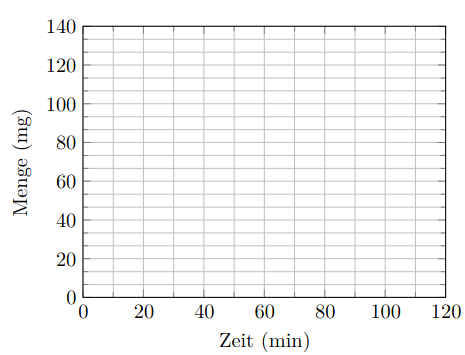
\includegraphics[width=150mm]{img/fct/Fct_ssA49.png}


c) Nach wie vielen Minuten ist die halbe Sättigungsmenge erreicht?
}{%% Lösung

a) $f(0) = 0$ mg

   $\lim_{x\rightarrow\infty} (f(x)) = 125 $ mg  ($\lim$ = limes =
   Limite hier für $x$ gegen unendlich.)

b) Grafik:

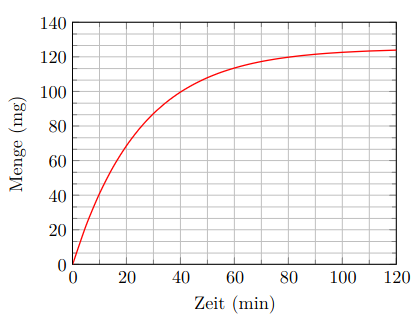
\includegraphics[width=150mm]{img/fct/Fct_ssL49.png}


c) Nach ca. 17.33 Minuten.

}{8}





\kNiveauAufgabe{
Die Anzahl mg eines durch Infusion verabreichten Medikaments im Blut verläuft gemäss der
Funktion ($x$ = Anzahl Stunden ab Infusionsbeginn, $y$ = Anzahl mg Medikament im Blut):

$$f : y = -250 \cdot{} e^{-0.2\cdot{}x} + 250$$


a) Stellen Sie die Funktion grafisch dar ($0 \le x \le 24$).

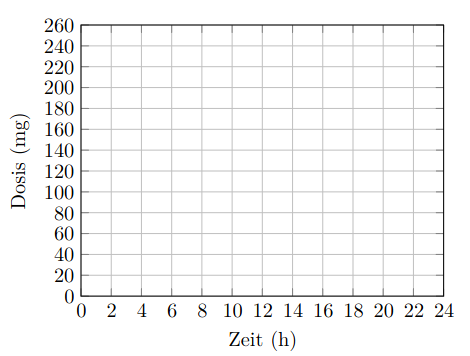
\includegraphics[width=150mm]{img/fct/Fct_ssA50.png}


b) Wie gross sind die $y$-Werte nach 3 und nach 4 Stunden ab
Infusionsbeginn?

c) Bei einer Dosis von 200 mg beginnt die Patientin plötzlich allergisch zu reagieren, worauf
die Infusion abgebrochen werden muss. Nach wie vielen Stunden ab Infusionsbeginn ist
dies der Fall?

}{%% Lösungen

a)
Grafik:

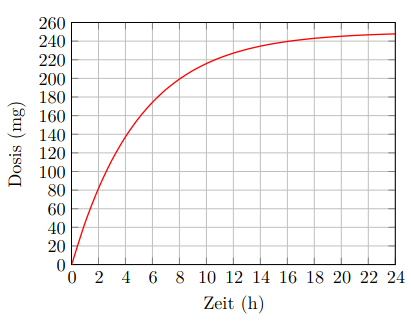
\includegraphics[width=150mm]{img/fct/Fct_ssL50.png}

b) $f(3)\approx 113$ mg \hspace{4cm}  $f(4) \approx{} 138$ mg

c) Nach 8.043 Stunden.
 
}{8}


\newpage
